\documentclass{article}
\usepackage{url}
\usepackage{graphicx} % To include figures
\usepackage{caption}
\usepackage{fullpage}
\usepackage{subcaption}
\usepackage{fancyvrb} % Includes the \VerbatimInput command to read in code files

\graphicspath{ {images/} }

% A very simple environment for writing pseudo-code
\newenvironment{pgm}{
  \begin{center}\begin{tabbing}
  xx \= xx \= xx \= xx \= xx \= xx \= xx \= xx \= xx \= xx \= xx \= \kill\>\+}{
  \end{tabbing}\end{center}}

\begin{document}
\begin{center}
	{\scshape \LARGE Examining New York City's Yellow Taxi Data Set \par}
	\vspace{0.3cm}
	{\scshape \large CS 516 Final Project - Midterm Report\par}
	\vspace{0.3cm}
	{ Ziyi \textsc{Wang}, Timothy \textsc{Blumberg}\par}
	\vspace{0.3cm}
	{ October 28, 2016\par}
	\vspace{1.5cm}
\end{center}



\section*{Abstract}

In our final project, we analyze NYC's {\textit very} public taxi dataset \cite{dataset} for interesting and surprising results. Our analysis has been principally done through queries on a SQL database, but because of the geographic nature of the data, we were forced to visualize from a very early stage in our project's formation. During this preliminary stage of developing our project, we have established an efficient workflow and found areas to engage in a more prolonged analysis during the remainder of the semester.

\section{The Data}
The dataset is extremely large (there is about $1.6$Gb of data produced every month at present date), so this creates many challenges as we attempt to gain insights from it. A powerful DBMS helps to cut down our query runtime considerably. The data is relatively clean given its size and complexity, and definitions for the coded portions of the data (such as the {\tt payment\_type} field) is given in the data dictionary \cite{dictionary}. The NYC Taxi \& Limousine Commission (TLC) collects and reports data for three different kinds of vehicles in NYC: yellow taxis, green taxis, and for-hire vehicles (FHV). Yellow taxis provide street-hailing service in Manhattan, Green taxis are designed to be useful when getting around in the boroughs of NYC, and the FHVs are available only through pre-arranging the pickup (i.e. cannot provide service that was not pre-arranged). For our project, we focus exclusively on the yellow taxis. \\

Each row contains start and end time, pickup and drop-off coordinates, number of passengers (as reported by the driver), fare amount, tip amount, distance traveled and several others. We took a look at many of the fields individually as well as exploring relationships between several variables at a time.


\section{Data Processing}
The data was downloaded as .csv file, automatically by python script. After
that, we created python code to select the columns of interest, map the
loacation information(recorded by latitude and longitude) into geohash string,
creat frequency table for each locations and organize time format for
analysis. Of all the columns the original data, we focused on pickup/drop off
locations pickup/drop off time and fare/tip/total amount. 

\begin{figure}
\centering
\begin{subfigure}{.5\linewidth}
  \centering
  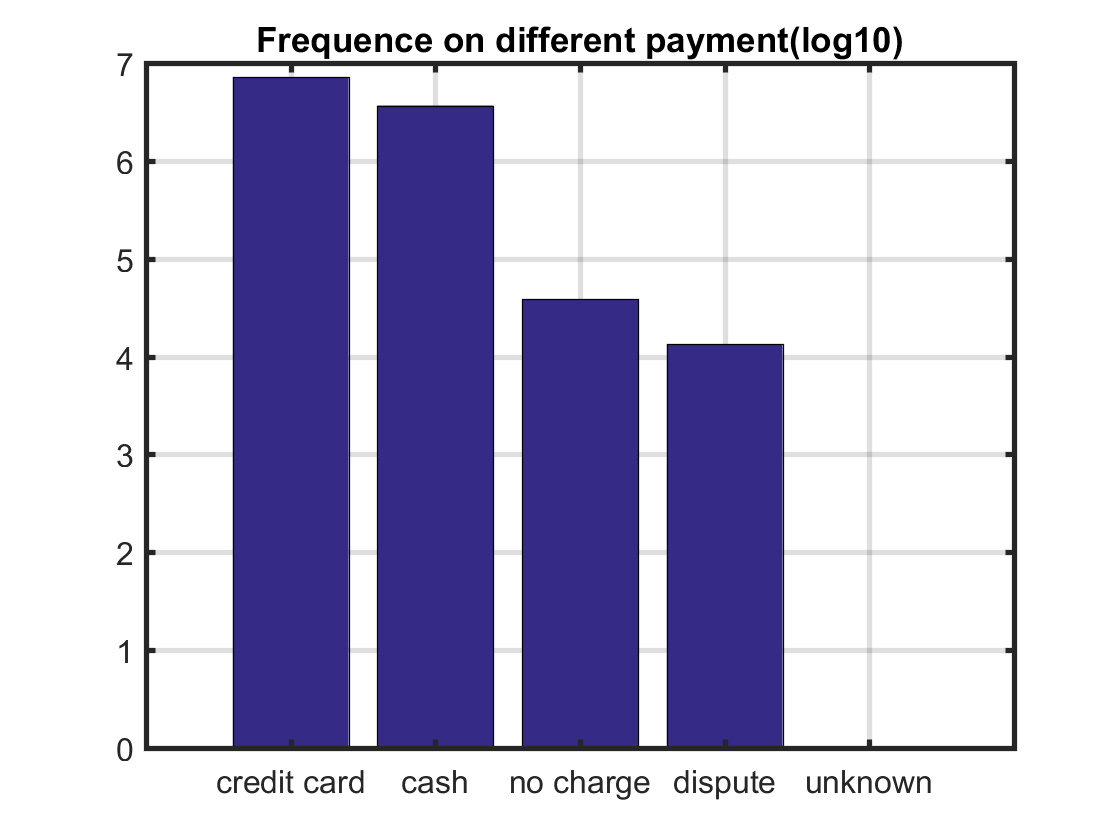
\includegraphics[width=.8\linewidth]{frequency-payment}
  \caption{Frequency of different payment methods}
  \label{fig:sub1}
\end{subfigure}%
\begin{subfigure}{.5\linewidth}
  \centering
  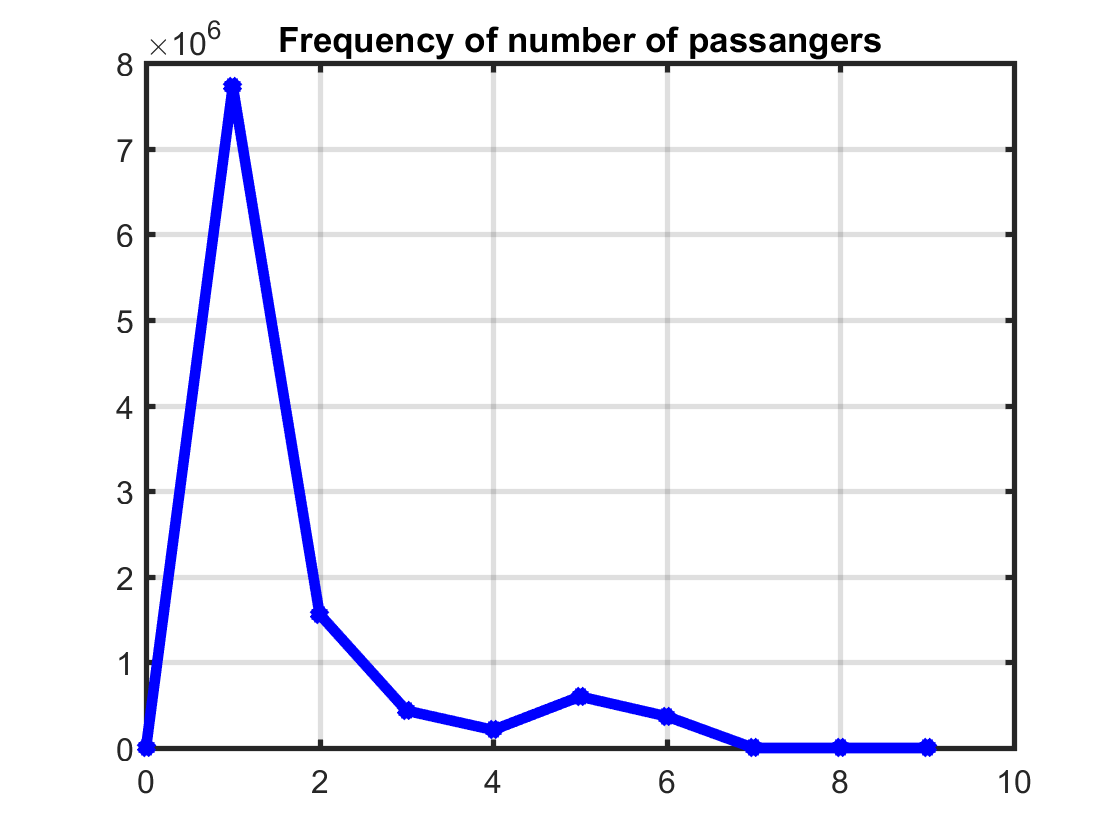
\includegraphics[width=.8\linewidth]{passange_frequency}
  \caption{Frequency of the number of passangers}
  \label{fig:sub2}
\end{subfigure}

\begin{subfigure}{.5\linewidth}
  \centering
  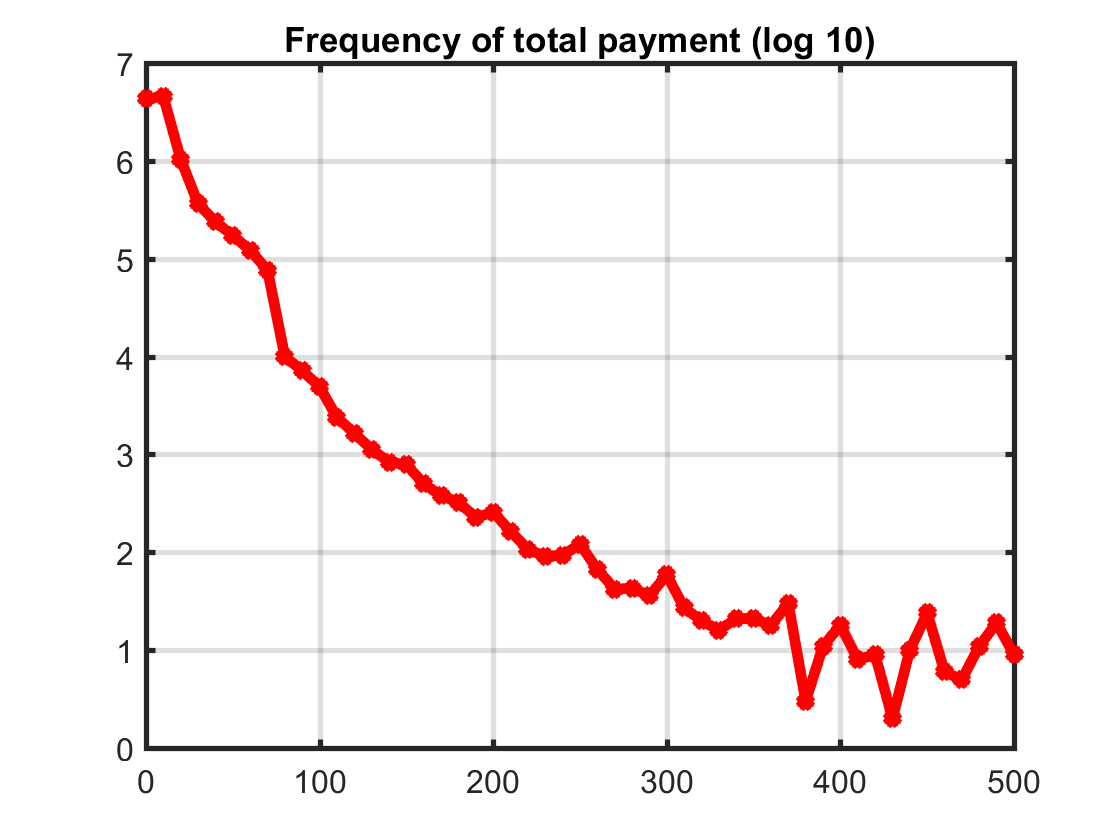
\includegraphics[width=.8\linewidth]{frequency-totalpayment}
  \caption{Frequency of the total payment amount}
  \label{fig:sub3}
\end{subfigure}%
\begin{subfigure}{.5\linewidth}
  \centering
  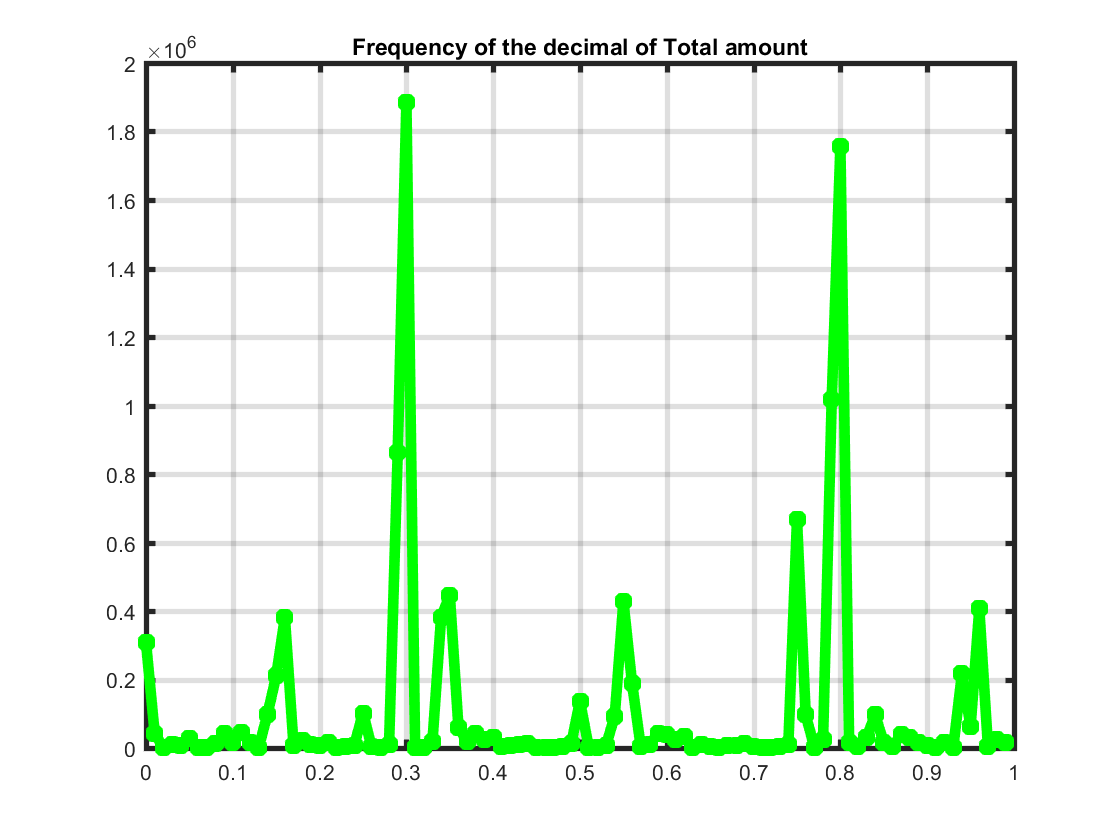
\includegraphics[width=.8\linewidth]{frequency-decimal-totalamount}
  \caption{Frequency of the decimal of total paymount amount}
  \label{fig:sub4}
\end{subfigure}

\begin{subfigure}{.5\linewidth}
  \centering
  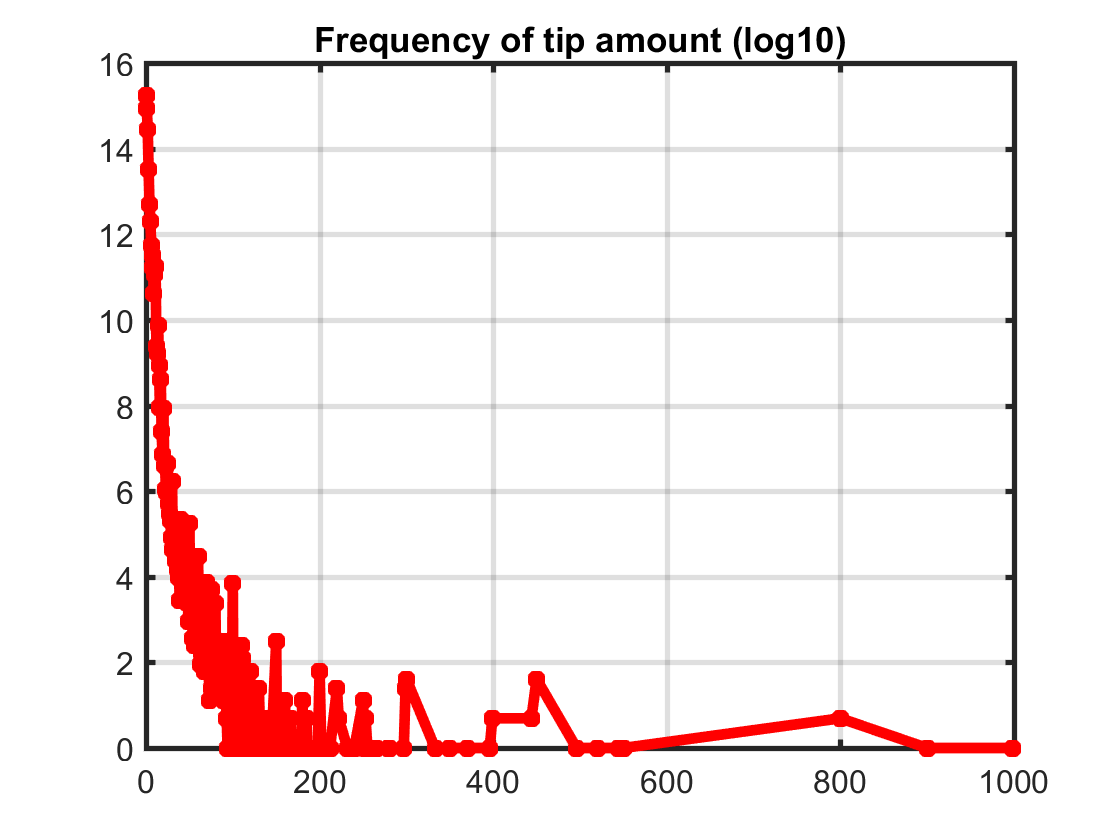
\includegraphics[width=.8\linewidth]{frequency-tipamount}
  \caption{Frequency of the tip amount}
  \label{fig:sub5}
\end{subfigure}%
\begin{subfigure}{.5\linewidth}
  \centering
  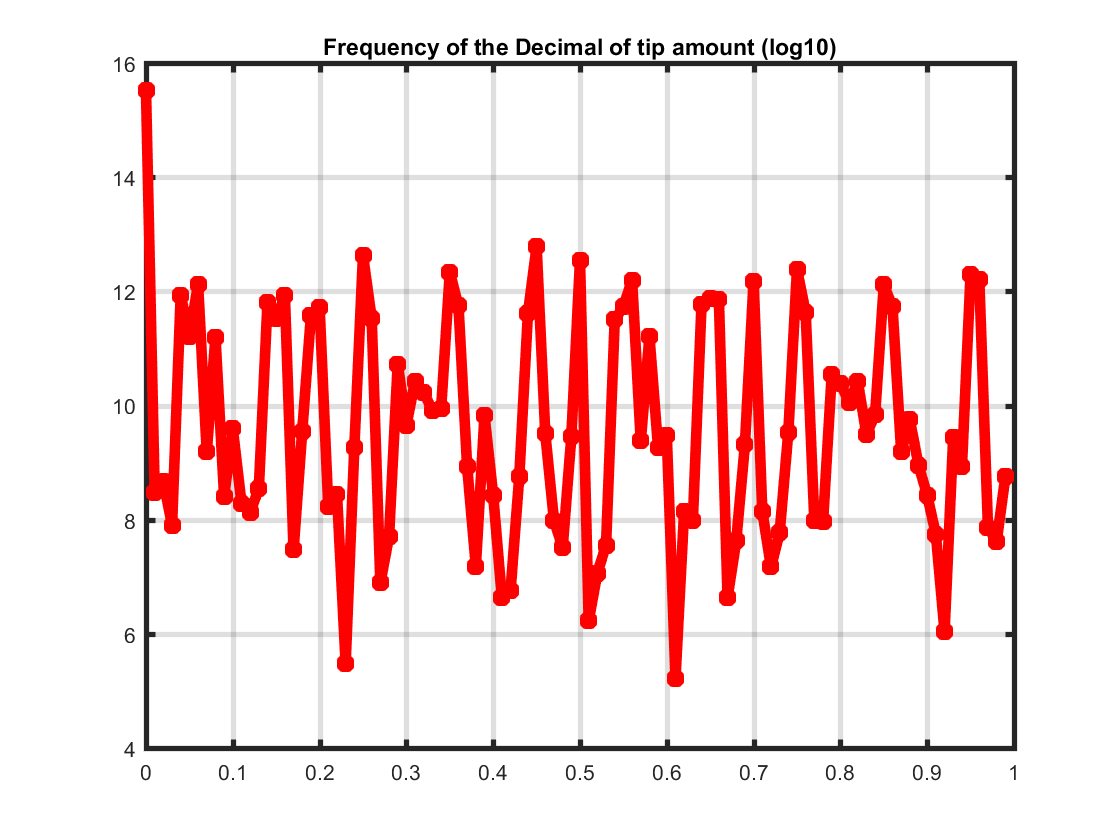
\includegraphics[width=.8\linewidth]{frequency-decimal-tipamount}
  \caption{Frequency of the decimal of tip amount}
  \label{fig:sub6}
\end{subfigure}

\begin{subfigure}{\linewidth}
  \centering
  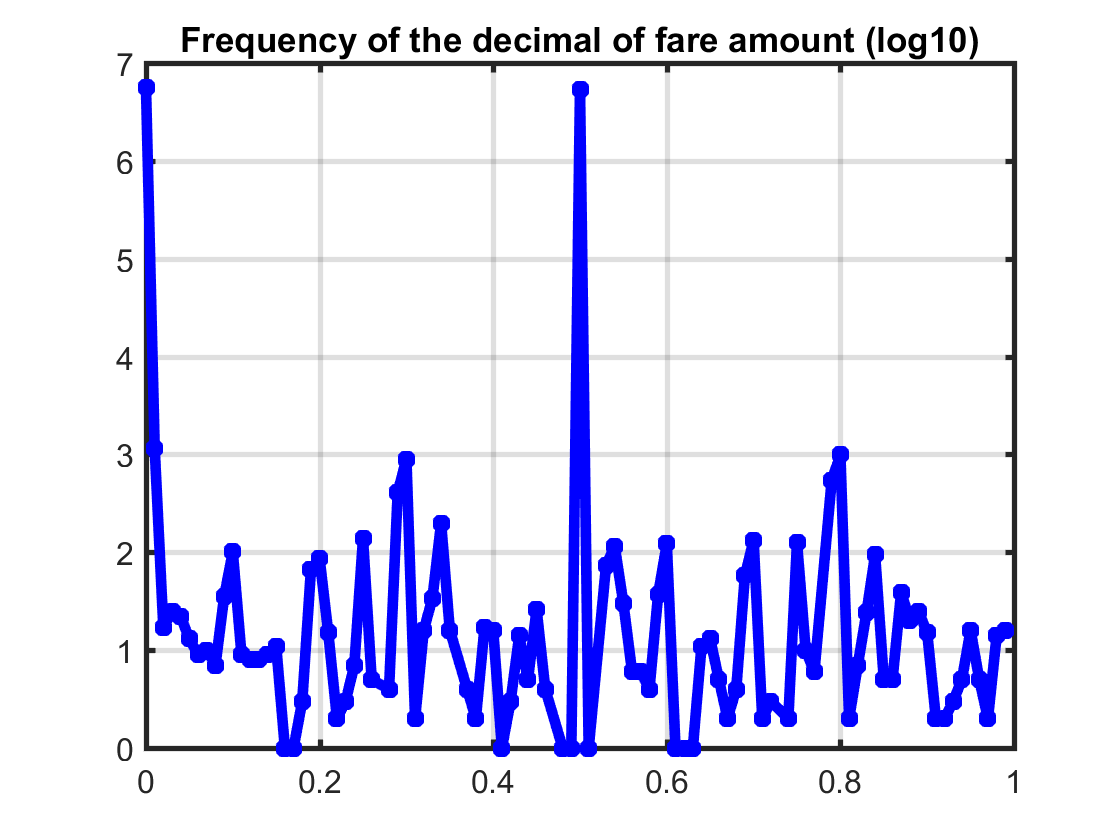
\includegraphics[width=.4\linewidth]{frequency-decimal-fareamount}
  \caption{Frequency of fare amount decimal}
  \label{fig:sub7}
\end{subfigure}
\caption{Statistics from passangers and fare}
\label{fig:test}
\end{figure}

\begin{figure}
\centering
\begin{subfigure}{.5\linewidth}
  \centering
  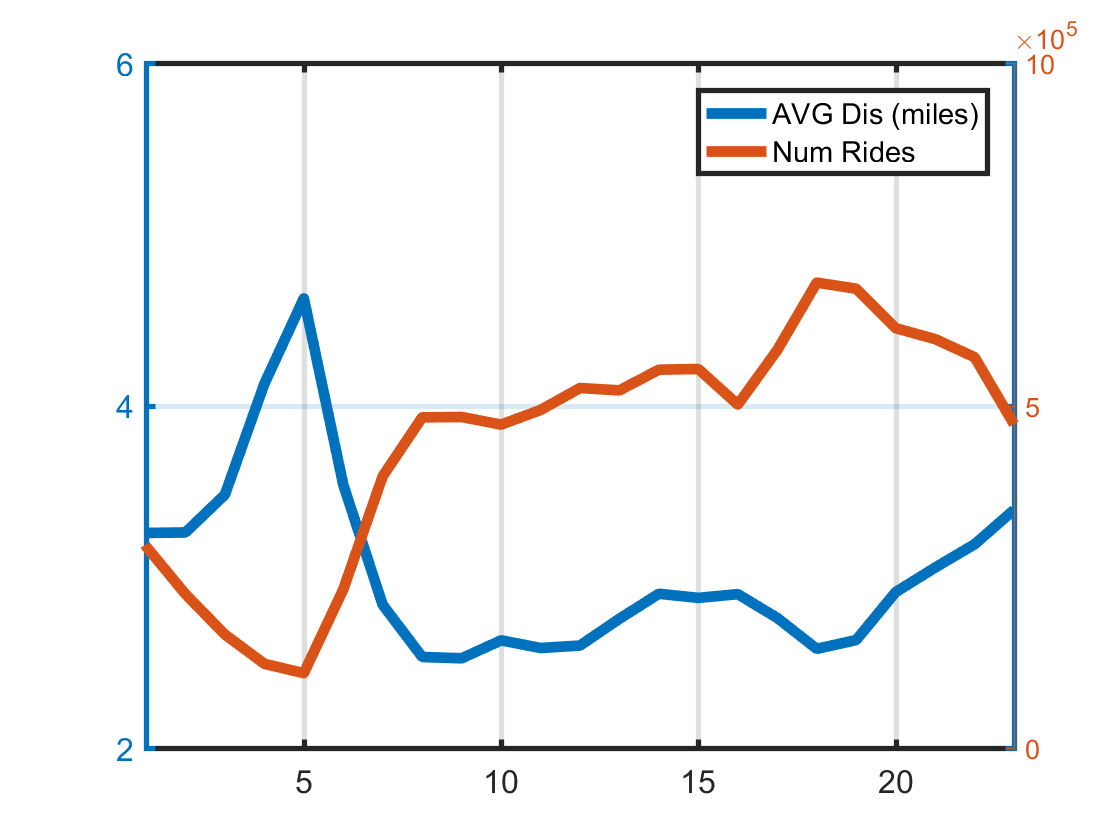
\includegraphics[width=.8\linewidth]{numride_tod}
  \caption{number of ride \& average distance (miles) in 24 hours}
  \label{fig:sub1}
\end{subfigure}%
\begin{subfigure}{.5\linewidth}
  \centering
  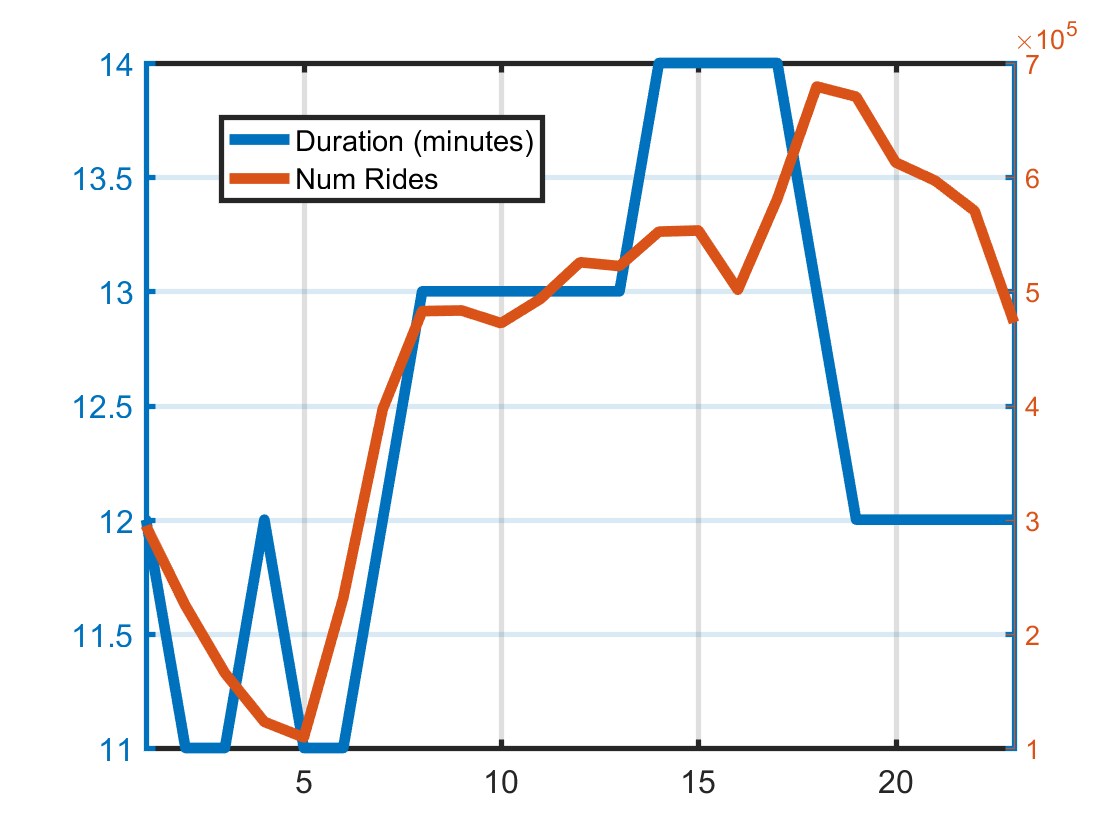
\includegraphics[width=.8\linewidth]{numride_tod_dur}
  \caption{number of ride \& average duration in (min) 24 hours}
  \label{fig:sub2}
\end{subfigure}

\begin{subfigure}{.5\linewidth}
  \centering
  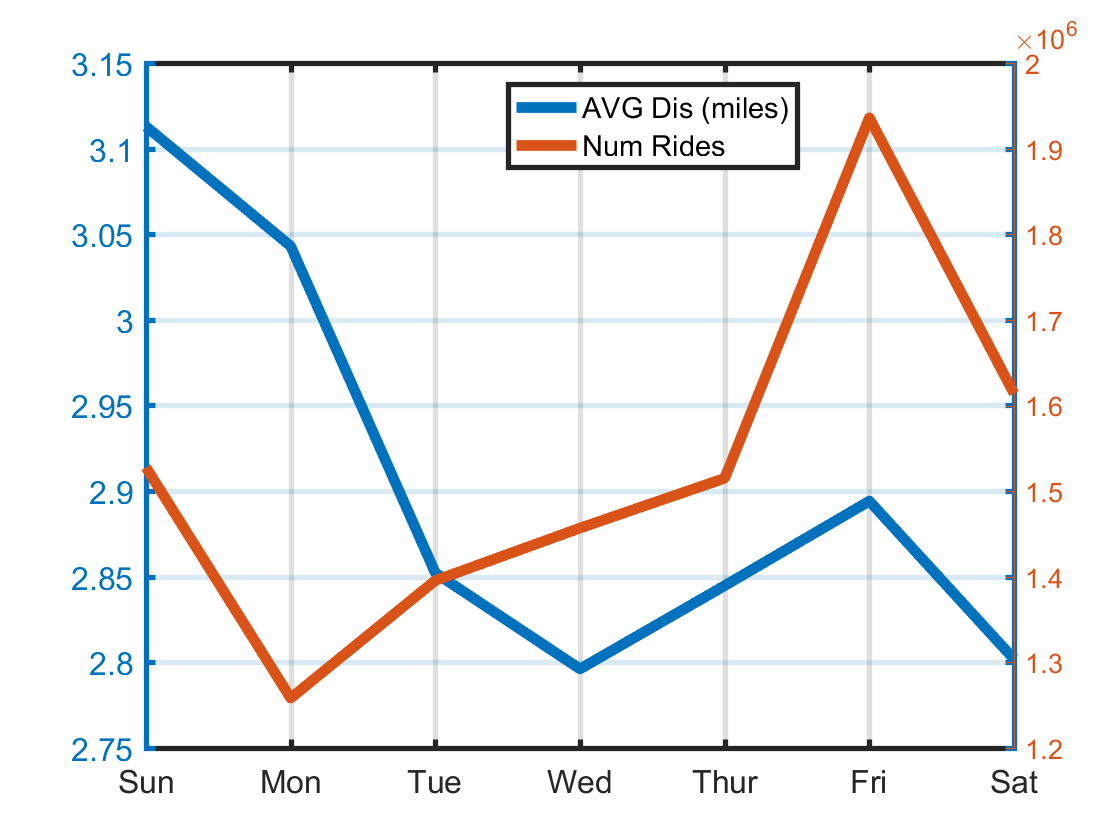
\includegraphics[width=.8\linewidth]{numride_dow}
  \caption{number of ride \& average distance (miles) in 7 days}
  \label{fig:sub3}
\end{subfigure}%
\begin{subfigure}{.5\linewidth}
  \centering
  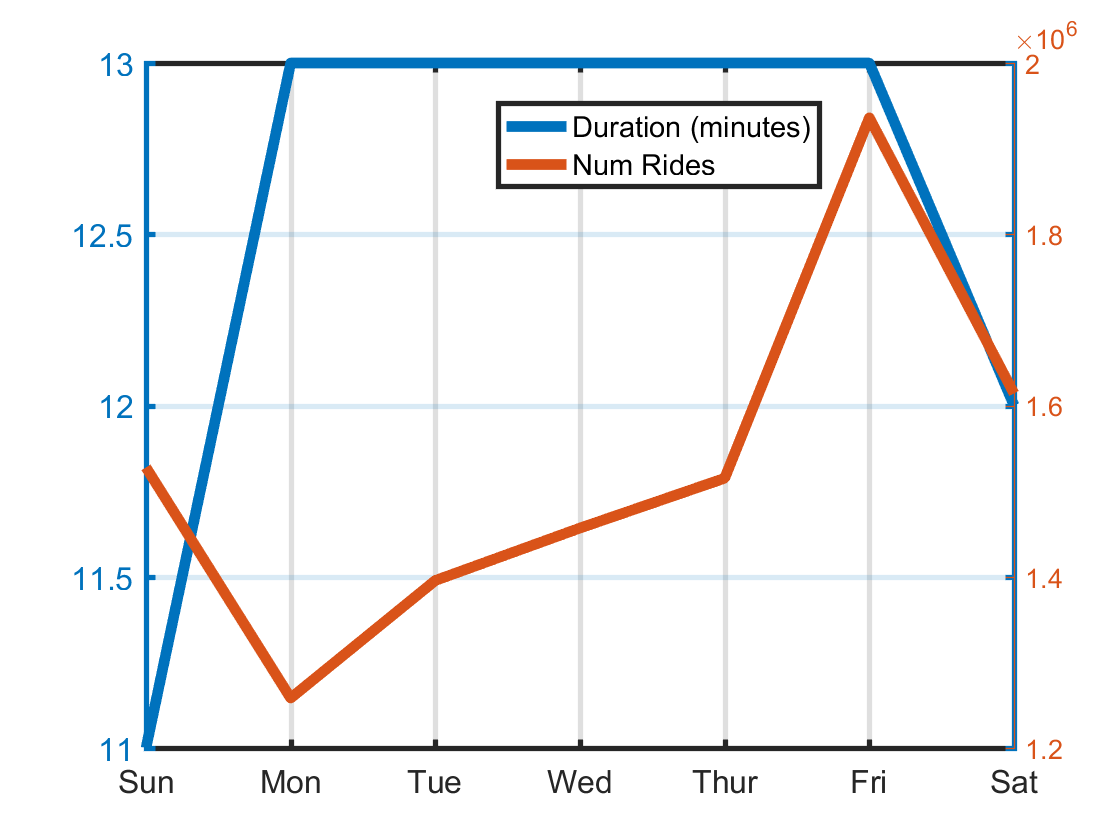
\includegraphics[width=.8\linewidth]{numride_dow_dur}
  \caption{number of ride \& average duration (min) in 7 days}
  \label{fig:sub4}
\end{subfigure}

\begin{subfigure}{.5\linewidth}
  \centering
  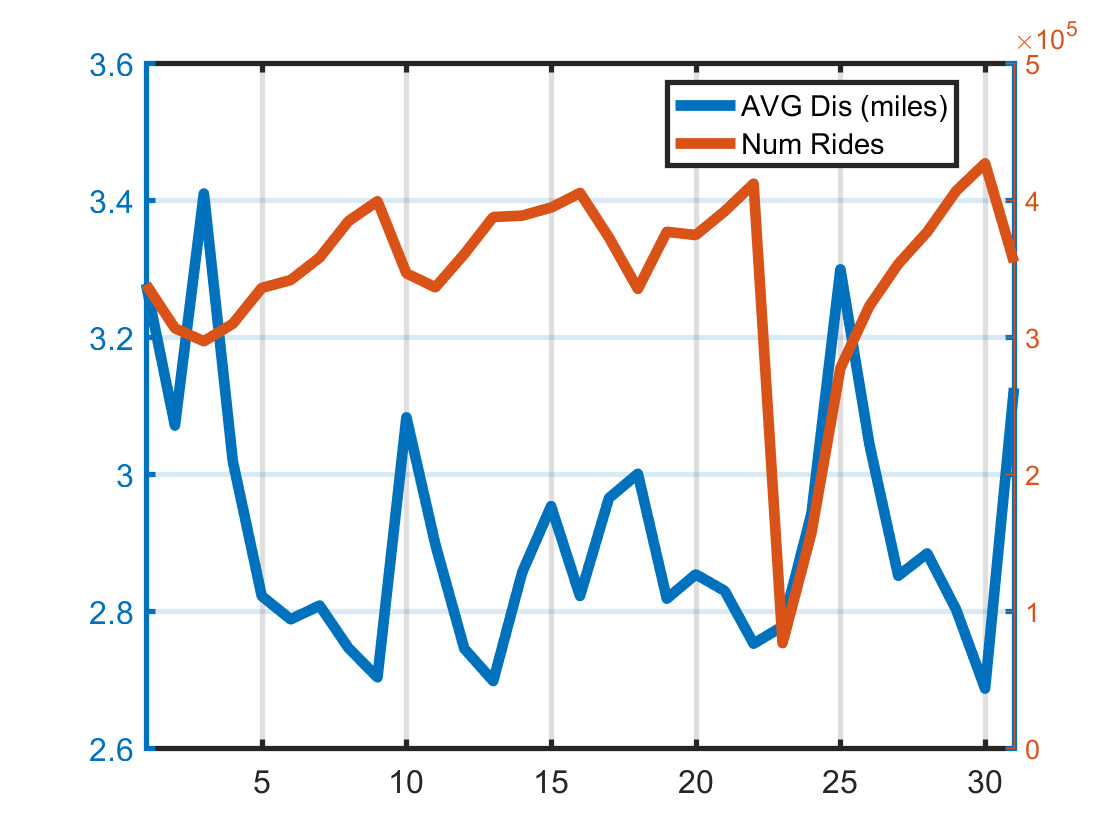
\includegraphics[width=.8\linewidth]{numride_dom}
  \caption{number of ride \& average distance (miles) in 31 days}
  \label{fig:sub5}
\end{subfigure}%
\begin{subfigure}{.5\linewidth}
  \centering
  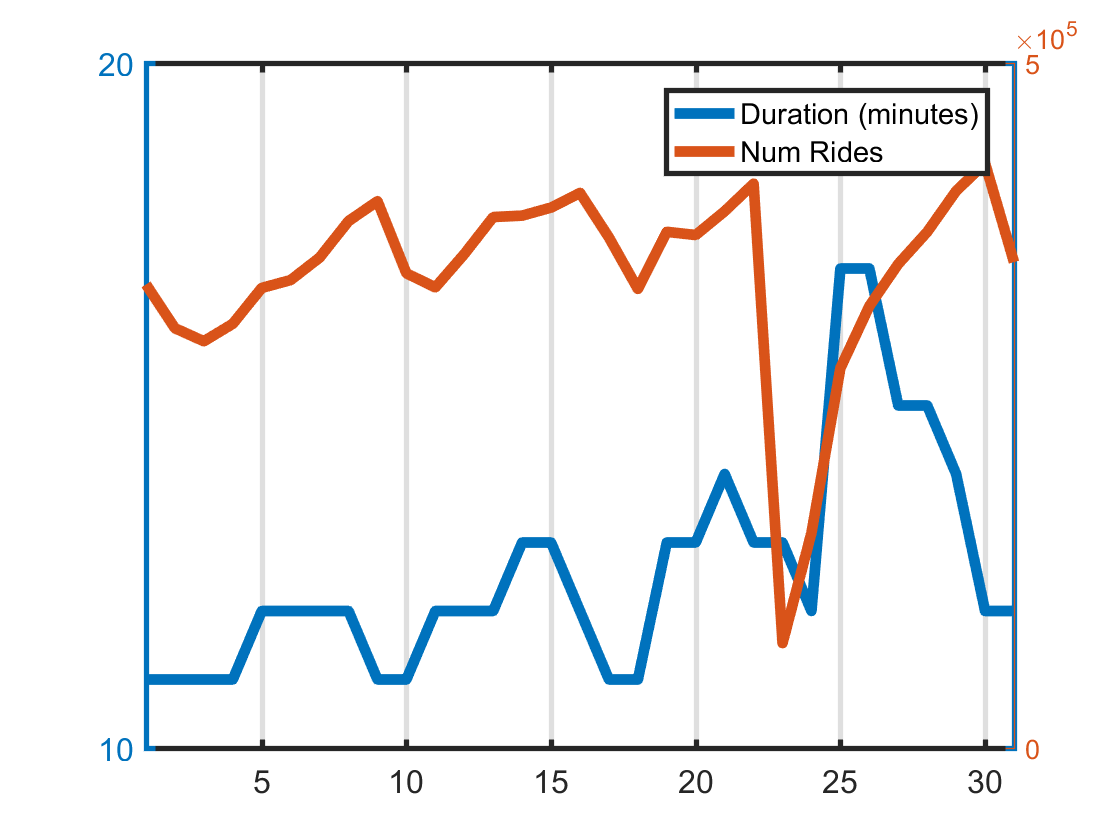
\includegraphics[width=.8\linewidth]{numride_dom_dur}
  \caption{number of ride \& average duration (min) in 31 days}
  \label{fig:sub6}
\end{subfigure}

\caption{Statistics from number of rides, distance and duration}
\label{fig:test}
\end{figure}

\section{Interesting Pieces of our Dataset}
\subsection{Statitics from the Data}
Figure 1 showes some statistics from the Dataset \cite{dataset}, from which we can find some interesting facts. (a) shows the frequency of payment methods used. Credit card was used the most frequently. No cash and dispute were also happening on a notable frequence. (b) shows the frequency of the number of passangers. From the subplot, we most of the case there was only one passanger in the taxi. (c) shows the frequency of different amount of payment. It is clear that as the total amount increases the frequency decreases. (d) shows the frequency of the decimal of the total fare amount. From the figure we see two clear peaks in $0.3$ and $0.8$, it is interesting that these two numbers are the most frequent decimal of the total amount. (e) shows the frequency of total amount of tips. (f) shows the frequency of the decimal of the tips. (g) shows the frequency of the decimal of total amount. It implies that people tend to round up the total amount to half dollar or a dollar. \\

Figure 2 showes the fluctuation of number of rides, average distance of rides and average duration, with respect to 24 hours in a day, 7 days in a week and 31 days in a month. The data is from 2016. The month plot used the data in Janurary. In the figure, each subfigure contains two plot with different Y scale. The left column is plotted with numbers of rides and average distance whereas the right column is numbers of rides and average duration. The three rows correspond to hours in a day, days in a week and days in a month. Column-wise, it shows that the average distance shows negative relation with number of rides, while average duration shows positive relation with number of rides. It is intuitive that with more rides, the traffic is heavier thus the average duration increases. It is relatively hard to interpret the negative correlation between number of rides and the average distance of rides. Another interesting finding is the plunge on number of riders around Jan. 23, in the plot of days in month (e,f). This was due to the blizzard happened on Jan. 22. It took couple days for the number of rides to recover after the blizzard. There are also two peaks occurred after the blizzard, on the average distance and average duration. It seems that after the blizzard, people traveled relatively farther and since more people were taking taxi, the traffic increase the average duration. 


\vfill

\medskip
\bibliographystyle{unsrt}
\bibliography{midterm_report}


\end{document}
\grid
\grid
\grid
